
\section{Factory Language (.fl) Updated}\label{appendix:factory-lang-updated}

\subsection{Metamodel}\label{appendix:metamodel-updated} 

\begin{figure}[H]
    \centering
    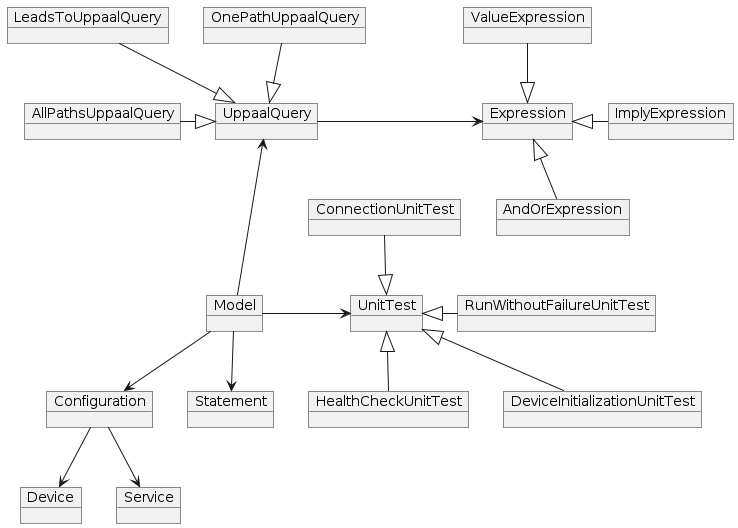
\includegraphics[width=.40\textwidth]{Image/metamodel-individual.png}
    \caption{An overview of the updated metamodel.}
    \label{fig:metamodel-updated}
\end{figure}

\subsection{Grammar Language}\label{appendix:grammar-language-updated}

\begin{minted}[breaklines]{python}
grammar xtext.factoryLang.FactoryLang with org.eclipse.xtext.common.Terminals

generate factoryLang "http://www.factoryLang.xtext/FactoryLang"

Model:
	'init' 'system' 'named' name=ID
	'CONFIGURATION:'
	BEGIN
	configuration=Configuration
	END
	'LOGIC:'
	BEGIN
	statements+=Statement*
	END
	'UNIT TESTS:'
	BEGIN
	unitTests+=UnitTest*
	END
	'UPPAAL QUERIES:'
	BEGIN
	uppaalQueries+=UppaalQuery*
	END;

// uppaalQueries+=UppaalQuery+;
// ----- CONFIGURATION ----- //
Configuration:
	{Configuration} services+=Service* devices+=Device*;

// ----- CONFIGURATION:SERVICE ----- //
Service:
	'define' serviceName=SERVICE_NAME 'named' name=ID 'with' address=Address ':' port=INT;

Address:
	ID ('.' ID)*;

// ----- CONFIGURATION:DEVICE ----- //
Device:
	'create' (Crane | Disk | Camera);

// ----- CONFIGURATION:CRANE ----- //
Crane returns Device:
	{Crane} 'crane' 'named' name=ID BEGIN targets+=CraneParameter+ END;

CraneParameter returns Parameter:
	CranePositionParameter;

CranePositionParameter returns CraneParameter:
	{CranePositionParameter} 'with' 'position' 'at' degree=INT 'named' name=ID;

// ----- CONFIGURATION:DISK ----- //
Disk returns Device:
	{Disk} 'disk' 'named' name=ID BEGIN slotParameter=DiskSlotParameter targets+=DiskParameter+ END;

DiskParameter returns Parameter:
	DiskZoneParameter;

DiskSlotParameter returns DiskParameter:
	{DiskSlotParameter} 'with' size=INT 'slots';

DiskZoneParameter returns DiskParameter:
	{DiskZoneParameter} 'with' 'zone' 'named' name=ID 'at' 'slot' slot=INT;

// ----- CONFIGURATION:CAMERA ----- //
Camera returns Device:
	{Camera} 'camera' 'named' name=ID BEGIN targets+=CameraParameter+ END;

CameraParameter returns Parameter:
	CameraColorParameter;

CameraColorParameter returns CameraParameter:
	{CameraColorParameter} 'with' 'scannable' 'color' color=COLOR;

// ----- STATEMENTS ----- //
Statement:
	Conditional | Operation | Loop;

// ----- STATEMENTS:CONDITIONALS ----- //
Conditional returns Statement:
	DeviceConditional | VariableConditional;

DeviceConditional returns Conditional:
	{DeviceConditional} 'if' 'device' device=[Device] 'is' (not_operator='not')? ('at')?
	deviceValue=DeviceValue
	'then' BEGIN statements+=Statement* END;

VariableConditional returns Conditional:
	{VariableConditional} 'if' 'variable' variable=[Variable] 'is'
	(comparison_operator=COMPARISON_OPERATOR)?
	variableValue=VariableValue
	'then' BEGIN statements+=Statement* END;

// ----- STATEMENTS:OPERATIONS ----- //
Operation returns Statement:
	CraneOperation | DiskOperation | CameraOperation;

// ----- STATEMENTS:OPERATIONS:CRANE ----- //
CraneOperation returns Operation:
	CranePickupOperation | CraneDropOperation;

CranePickupOperation returns CraneOperation:
	{CranePickupOperation} device=[Crane] 'pickup' 'item' 'at' target=[CraneParameter];

CraneDropOperation returns CraneOperation:
	{CraneDropOperation} device=[Crane] 'drop' 'item' 'at' target=[CraneParameter];

// ----- STATEMENTS:OPERATIONS:DISK ----- //
DiskOperation returns Operation:
	DiskMoveEmptySlotOperation | DiskMoveVariableSlotOperation | DiskMoveSlotOperation | DiskMarkSlotOperation |
	DiskWaitOperation;

DiskMoveSlotOperation returns DiskOperation:
	{DiskMoveSlotOperation} device=[Disk] 'move' 'slot' 'at' source=[DiskZoneParameter] 'to'
	target=[DiskZoneParameter];

DiskMoveVariableSlotOperation returns DiskOperation:
	{DiskMoveVariableSlotOperation} device=[Disk] 'move' 'slot' 'of' variable=[Variable] 'to'
	target=[DiskZoneParameter];

DiskMoveEmptySlotOperation returns DiskOperation:
	{DiskMoveEmptySlotOperation} device=[Disk] 'move' 'empty' 'slot' 'to' target=[DiskZoneParameter];

DiskMarkSlotOperation returns DiskOperation:
	{DiskMarkSlotOperation} device=[Disk] 'mark' 'slot' 'at' target=[DiskZoneParameter] 'as'
	diskSlotValue=DiskSlotValue ('in' quantity=INT measure=TIME)?;

DiskWaitOperation returns DiskOperation:
	{DiskWaitOperation} device=[Disk] 'wait' 'for' 'new' 'item';

// ----- STATEMENTS:OPERATIONS:CAMERA ----- //
CameraOperation returns Operation:
	CameraScanOperation;

CameraScanOperation returns CameraOperation:
	{CameraScanOperation} device=[Camera] 'scan' 'color' 'into' variable=GlobalVariable;

// ----- STATEMENTS:LOOPS ----- //
Loop returns Statement:
	ForEach;

// ----- STATEMENTS:LOOPS:FOREACH ----- //
ForEach returns Loop:
	{ForEach} 'for' 'each' variable=LocalVariable 'in' device=[Device] 'that' 'is' (operator='not')?
	variableValue=VariableValue
	'then' BEGIN statements+=Statement* END;

// ----- UnitTests ----- //
UnitTest:
	HealthCheckUnitTest | ConnectionUnitTest | DeviceInitializationUnitTest | RunWithoutFailureUnitTest;

HealthCheckUnitTest returns UnitTest:
	{HealthCheckUnitTest} 'test' service=[Service] 'and' 'assert' 'health status' 'is' status=STATUS;

ConnectionUnitTest returns UnitTest:
	{ConnectionUnitTest} 'test' service=[Service] 'and' 'assert' 'connection' 'is' status=STATUS;

DeviceInitializationUnitTest returns UnitTest:
	{DeviceInitializationUnitTest} 'test' devices+=[Device] (',' devices+=[Device])* 'and' 'assert' ('device' |
	'devices') ('is' | 'are') 'initialized';

RunWithoutFailureUnitTest returns UnitTest:
	{RunWithoutFailureUnitTest} 'test' application=[Model] 'and' 'assert' 'it' 'runs';

// ----- UppaalQueries ----- //
UppaalQuery:
	AllPathsUppaalQuery | OnePathUppaalQuery | LeadsToUppaalQuery;

AllPathsUppaalQuery returns UppaalQuery:
	{AllPathsUppaalQuery} 'query' 'that' property=('forever' | 'eventually') 'on' 'all' 'paths' '(' BEGIN not=('not')?
	expression=AndOrExpression END ')';

OnePathUppaalQuery returns UppaalQuery:
	{OnePathUppaalQuery} 'query' 'that' property=('forever' | 'eventually') 'on' 'one' 'path' '(' BEGIN not=('not')?
	expression=AndOrExpression END ')';

LeadsToUppaalQuery returns UppaalQuery:
	{LeadsToUppaalQuery} 'query' 'that' '(' BEGIN not1=('not')? stateOne=ValueExpression 'leads' 'to' not2=('not')?
	stateTwo=ValueExpression END ')';

AndOrExpression returns Expression:
	ImplyExpression (({Or.left=current} 'or' | {And.left=current} 'and') not=('not')? right=ImplyExpression)*;

ImplyExpression returns Expression:
	ValueExpression (({Imply.left=current} 'imply') not=('not')? right=ValueExpression)*;

ValueExpression returns Expression:
	{Parenthesis} '(' parenthesizedExpression=AndOrExpression ')' | DeviceState;

DeviceState:
	device=[Device] '.' location=ID;

// ----- VARIABLES ----- //
LocalVariable returns Variable:
	{LocalVariable} name=ID;

GlobalVariable returns Variable:
	{GlobalVariable} name=ID;

// ----- VALUE TYPES ----- //
DeviceValue:
	value=DiskStateValue | value=ColorValue | ref=[Parameter];

DiskSlotValue:
	value=DiskSlotStateValue | value=ColorValue | ref=[Variable];

VariableValue:
	value=DiskSlotStateValue | value=ColorValue | value=Number | value=DiskStateValue | ref=[Variable];

// ----- VALUE TYPES:ACTUAL VALUES ----- //
DiskStateValue:
	value=DISK_STATES;

DiskSlotStateValue:
	value=DISK_SLOT_STATES;

ColorValue:
	value=COLOR;

Number:
	value=INT;

// ----- SHARED ENUMS ----- //
enum COMPARISON_OPERATOR:
	UNDEFINED='undefined' | LESS_THAN='less than' | GREATER_THAN='greater than' | NOT='not';

enum COLOR:
	RED='red' | GREEN='green' | BLUE='blue';

enum DISK_SLOT_STATES:
	FREE='free' | IN_PROGRESS='in_progress' | COMPLETE='complete';

enum DISK_STATES:
	FULL='full' | EMPTY='empty';

enum TIME:
	SECONDS='seconds' | SECOND='second' | MINUTES='minutes' | MINUTE='minute' | HOURS='hours' | HOUR='hour';

enum SERVICE_NAME:
	MQTT='mqtt' | DATABASE='database';

enum STATUS:
	UP='up' | DOWN='down';

// ----- TERMINALS ----- //
terminal BEGIN:
	'synthetic:BEGIN';

terminal END:
	'synthetic:END';
\end{minted}

\subsection{Example Factory Language program}\label{appendix:fl-updated}
\begin{minted}[breaklines]{python}
init system named OrchestratorService

CONFIGURATION:
	define mqtt named ^mqtt with ^test.mosquitto.org:1883
	define database named influxdb with influxdb.devantler.com:8086
	
	create crane named crane1
		with position at 0 named intake 
		with position at 40 named outRed 
		with position at 55 named outGreen 
		with position at 70 named outBlue  
	
	create disk named disk1
		with 4 slots
		with zone named craneZone  at slot 1 
		with zone named cameraZone at slot 2
		with zone named intakeZone at slot 3 
	
	create camera named camera1
		with scannable color blue 
		with scannable color green 
		with scannable color red

LOGIC:
	for each diskSlot in disk1 that is complete then
		disk1 move slot of diskSlot to craneZone
		crane1 pickup item at intake
		disk1 mark slot at craneZone as free
		if variable diskSlot is red then  
			crane1 drop item at outRed
		if variable diskSlot is green then  
			crane1 drop item at outGreen
		if variable diskSlot is blue then  
			crane1 drop item at outBlue
	
	if device disk1 is not full then  
		disk1 move empty slot to intakeZone
		disk1 wait for new item
		disk1 mark slot at intakeZone as in_progress 
		disk1 move slot at intakeZone to cameraZone
		camera1 scan color into currentItemColor 
		disk1 mark slot at cameraZone as currentItemColor  
		if variable currentItemColor is red then  
			disk1 mark slot at cameraZone as complete in 10 seconds  
		if variable currentItemColor is green then  
			disk1 mark slot at cameraZone as complete in 20 seconds  
		if variable currentItemColor is blue then  
			disk1 mark slot at cameraZone as complete in 30 seconds

UNIT TESTS:
	test ^mqtt and assert health status is up
	test ^mqtt and assert connection is up
	test influxdb and assert health status is down
	test influxdb and assert connection is down
	test camera1, crane1, disk1 and assert devices are initialized
	test OrchestratorService and assert it runs
	
UPPAAL QUERIES:
	//A[] (disk1.Position1 imply (disk1.Position1 or disk1.Position2 or disk1.Position3))
	query that forever on all paths (
		disk1.Position1 imply (disk1.Position1 or disk1.Position2 or disk1.Position3)
	)
	
	//A<> (disk1.Stopped and crane1.crane1_Stopped) imply (disk1.Position1 and crane1.crane1_Stopped)
	query that eventually on all paths (
		(disk1.Stopped and crane1.Stopped) imply (disk1.Position1 and crane1.Stopped)
	)
	
	//E[] (disk1.Position1 or disk1.Position2 or disk1.Position3 or disk1.Position4)
	query that forever on one path (
		disk1.Position1 or disk1.Position2 or disk1.Position3 or disk1.Position4
	)
	
	//E<> (disk1.Position1 imply disk1.Position2)
	query that eventually on one path (
		disk1.Position1 imply disk1.Position2
	)
	
	//camera1.camera1_Green --> camera1.camera1_Idle
	query that (
		camera1.camera1_Green leads to camera1.camera1_Idle
	)
	
	//Just a test to show negation works
	query that eventually on all paths (
		not camera1.dsd or not disk1.sds
	)
\end{minted}
